\documentclass{article}
    \usepackage{ctex}
    \usepackage{algorithm}
    \usepackage{algorithmicx}
    \usepackage{algpseudocode}
    \usepackage{graphicx}
    \floatname{algorithm}{算法}
    \renewcommand{\algorithmicrequire}{\textbf{输入:}}
    \renewcommand{\algorithmicensure}{\textbf{输出:}}
    \title{视频字幕识别项目文档}
    \author{同济大学}
    \date{\today}
    
    \begin{document}
        \maketitle
        \section{简介}
        本项目基于OpenCV以及Azure的OCR服务,
        成功完成了任务。

        程序分为两部分:
        \begin{itemize}
            \item 基于OpenCV的字幕提取:利用多线程,使得读取视频和提取字幕并行;
            \textbf{在提取字幕方面,我们开发了一种算法,能够很好地剔除重复、
            无关的帧,提取出含有字幕的帧,并能滤掉背景(使成黑色),仅使字幕(白色)清晰显示。}
            \item 基于Azure的OCR:读取上一步得到的图片文件,
            返回识别结果.
        \end{itemize}

        实践证明,我们的算法不仅性能优越,同时也得到了很好的结果。\textbf{
            precision最高达到了100\%,且recall也能接近99\%。处理接近3小时的电影,
        提取字幕仅用时12分钟。}
        
        \section{使用说明}
        Windows环境下在powershell下运行

        > ./run.exe  your\_vedio\_path  subtitle\_save\_path

        需要输入两个路径:
        \begin{itemize}
            \item 视频的存放路径
            \item 字幕的存放路径
        \end{itemize}

        然后调用OCR.py启动Azure的OCR服务。
        \section{算法原理}
            \subsection{字幕区域识别}
                我们采用传统的图像处理方法,
                能够很好的识别并定位出字幕的区域,
                同样也能判断是否存在字幕。

                我们的算法可以用下面伪代码描述(为了清晰起见,调用函数的名称与MATLAB函数或者
                OpenCV函数一致):
                \begin{algorithm}
                    \caption{字幕区域识别}
                    \begin{algorithmic}[1]
                        \Require 视频某帧图片
                        \Ensure 判断是否存在字幕,如果存在并返回处理后的含字幕图片
                        \Function {SubtitleLocating}{$input\_img, output\_img$}
                            \State $Let\quad temp\_img\quad be\quad  new\quad  matrix$
                            \State $temp\_img \gets \Call{rgb2gray}{input\_img}$
                            \State $temp\_img \gets \Call{imadjust}{temp\_img}$
                            \State $output\_img \gets \Call{imopen}{temp\_img}$
                            \State $output\_img \gets \Call{imsubstract}{temp\_img, output\_img}$
                            \State $output\_img \gets \Call{imopen}{output\_img}$
                            \State $output\_img \gets \Call{imclose}{output\_img}$
                            \State $Let\quad contours\quad be\quad new\quad vector\quad of\quad Points$
                            \State $contours \gets \Call{findContours}{output\_img} $
                            \State $has\_caption \gets False$
                            \For{$i = 0 \to contours.size$}
                                \State $rect \gets \Call{boudingRect}{contours[i]}$
                                \If{$the\quad rect\quad is\quad at\quad center$}
                                    \State $has\_caption \gets True$
                                    \State $ output\_img(rect) \gets temp\_img(rect) $
                                \Else
                                    \State $ output\_img(rect) \gets Black$
                                \EndIf
                            \EndFor
                            \State \Return{$has\_caption$} 
                        \EndFunction
                    \end{algorithmic}
                \end{algorithm}


                算法的第3-6行,是本算法的核心内容。经过第3行的灰度化后,第4行的imadjust图像增强
                是为了将图片的灰度映射到更紧密的一个范围中去,方便下面的处理,实践证明这一步对结果
                是有举足轻重的作用的。第5行的imopen形态学开操作,是该算法的精髓。这一步可以将字幕
                区域模糊化,甚至可以做到直接融于背景色中。所以通过最后一步,也就是第六行的差分操作,
                就可以轻松得到清晰的字幕。其实大多数视频帧做到这一步,效果已经非常好了。

                算法的7-21行,是进一步滤掉背景噪声,得到更为干净的字幕。首先通过算法第7-8行
                的形态学开操作和闭操作,使得字幕的区域能连通成一体。然后通过9-10行的一个
                寻找连通区域的函数,经过筛选,就可以锁定字幕所在的连通区域。我们确立了三条
                筛选的原则:一是连通区域的平均水平位置是在中央附近50像素以内;
                二是连通区域的底部不高于图片底部30像素;三是连通区域大小必须超过4000.
                如果没有任何一个连通区域,或者不满足上述任一条件,那么判定为该图片不存在字幕,同时把
                不符合要求的区域变成黑色;
                若存在一个区域能满足上述所有条件,那么满足的区域就是字幕所在区域。这样,就得到了干净的字幕。


            \subsection{字幕去重}
                我们采取的提取策略是每20帧提取一张图片进行处理,其余的全都忽略。
                但是很多时候,一条字幕会跨很多帧。这样势必要解决一个去重的问题。

                我们的解决策略是计算上一张处理后的字幕图片与当前处理后的字幕图片
                的余弦相似度,
                \begin{equation}
                    cosine = \frac{dot(A,B)}{norm2(A)*norm2(B)}
                \end{equation}

                我们判定,$cosine > 0.5$的视为两张图片相同;$cosine < 0.5$的
                视为两张图片不同。因为我们滤掉了背景,所以这种方法对于字幕去重
                极为有用。
                那么,每当出现前一张和当前这张图片计算余弦相似度,
                出现$cosine < 0.5$的情况,那么就保存当前这张图片;反之认为图像一致,
                不进行保存。这样就完成了字幕的去重。
            \subsection{生产者-消费者模型}
                为了提高程序的效率,我们并不是等视频处理函数读取完每帧图片后
                再进行处理,而是边读取视频,边处理图片。我们采用了著名的生产者-
                消费者模型。

                我们设置了一个队列,保存图片的矩阵头信息(OpenCV中的Mat)。
                同时开了两个线程,一个读取视频流,每二十帧将图片的矩阵头压入队列中,此为生产者;
                另一个线程进行从队列中取矩阵头,处理图片,此为消费者。

                为了防止多线程同时访问共享资源,我们设置了锁。利用C++11的unique\_lock
                和condition\_variable,可以保证队列线程安全。

        \section{性能与效果}
            示例:
            \begin{figure}[!hbp]
                \centering
                
\includegraphics[scale=0.3]{img_80420.jpg}
                \caption{原图}
            \end{figure}
            
            \begin{figure}[!hbp]
                \centering
                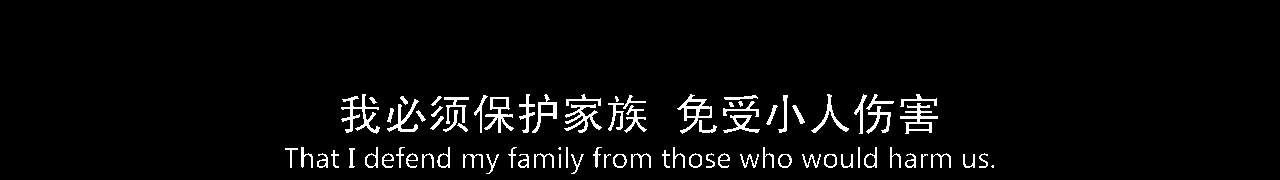
\includegraphics[scale=0.3]{604.png}
                \caption{提取图}
            \end{figure}
            
            更多图片请见附件.

            性能上,我们对很多视频的字幕提取进行了测速,得到了一个平均值:
            每秒钟处理能力为390帧左右。6分钟就能处理完1h30m的视频(配置:i7-6700)。

            效果上,除非是由于字幕出现不足20帧因而被略过的缘故,一般都能
            找到所有字幕。但是也会掺杂不是字幕的图片,不过一般这些“杂质”
            不能识别,因此对识别的结果不会产生影响。

            识别结果见附件output.txt.
    \end{document}